\chapter{مقدمه}
\noindent
\textbf{
\textit{
توضیحی اولیه مشتمل بر تعریف الگوریتم، نحوه کلی عملکرد الگوریتم، پایه‌های ریاضی، کاربردها و استانداردها
}
}
\pagebreak
\section{توضیح الگوریتم}
\par
الگوریتمی که در ادامهٔ این مستند شرح و توضیح آن آمده است الگوریتم درهم سازی 
\lr{skein}
یا 
\lr{skein hash function}
است. این الگوریتم از سری الگوریتم‌های درهم‌سازی امنیتی یا 
\lr{cryptographic hash function}
 و یکی از نامزدهای نهایی مسابقه انتخاب بهترین تابع درهم‌سازی 
 \lr{NIST}
 می‌باشد. این مسابقه برای انتخاب بهترین الگوریتم در‌هم‌سازی برای استاندارد جدید 
 \lr{SHA-3}
 برگزار شد. 
 طبق ادعای طراحان الگوریتم این الگوریتم می‌تواند در 
 \lr{6.1}
 کلاک در بایت داده‌ها را هش کند، که به این معنیست که در پردازندهٔ دوهسته‌ای
 \lr{64}
  بیتی با فرکانس پردازشی
\lr{3.1 GHz}
    می‌تواند با سرعت 
\lr{500}
  مگابایت بر ثانیه داده‌ها را هش کند. این مقدار سرعت تقریبا دوبرابر سرعت هش کردن دادهٔ الگوریتم 
  \lr{ SHA-512}
  است. همچنین با گزینه درخت درهم‌سازی که می‌تواند به صورت اختیاری در الگوریتم پیاده‌سازی شود می‌توان 	در پیاده‌سازی موازی الگوریتم سرعت را به بیش از این هم رساند. نکته دیگری که در مورد الگوریتم 
  \lr{skein}
  لازم به ذکر است این است که این الگوریتم پیاده‌سازی آسان و ساده‌ای دارد و فقط از سه عمل‌گر اصلی برای محاسبه هش استفاده می‌کند و نحوهٔ عملکرد الگوریتم به راحتی قابل به خاطرسپاری و یادگیری‌ست. 
  \par
  الگوریتم درهم‌سازی
  \lr{skein}
  برای حالت‌های ورودی ۲۵۶، ۵۱۲ و ۱۰۲۴ بایتی و هرمقداری خروجی پیاده‌سازی شده است که این خاصیت در انعطاف الگوریتم در حالت‌های مختلف بسیار حیاتی‌ست. 
  \\
  در پیاده‌سازی سخت‌افزاری نیز این الگوریتم قوی عمل می‌کند،‌برای پیاده‌سازی 
  \lr{skein-512}
  بر سخت‌افزار به حدود ۲۰۰ بایت فضای مموری نیاز داریم، برای 
  \lr{skein-256}
  این مفدار به حدود ۱۰۰ بایت کاهش پیاده می‌کند که این الگوریتم را به یک الگوریتم مناسب برای پیاده‌سازی‌های روی قطعات کوچک سخت‌افزاری تبدیل می‌کند، مثلا می‌توان از 
  \lr{skein-256}
  در پیاده‌سازی 
  \lr{smart card}
  استفاده کرد.
  \cite{skein}
 
  
  \subsection{مثال‌هایی از درهم‌سازی}

	\begin{itemize}
	
	\item \lr{Skein-256-256("")}\\
$c8877087da56e072870daa843f176e9453115929094c3a40c463a196c29bf7ba$
\item \lr{Skein-512-256("")}\\
$39ccc4554a8b31853b9de7a1fe638a24cce6b35a55f2431009e18780335d2621$
\item \lr{Skein-512-512("")}\\
$bc5b4c50925519c290cc634277ae3d6257212395cba733bbad37a4af0fa06af4$\\
$1fca7903d06564fea7a2d3730dbdb80c1f85562dfcc070334ea4d1d9e72cba7a$

	\end{itemize}
	
\section{مختصری دربارهٔ الگوریتم‌های درهم‌سازی امنیتی}
در دنیای امروز الگوریتم‌های درهم‌سازی امنیتی تقریبا در تمامی نقاط مختلفی که با اینترنت سر و کار دارند پیدا می‌شوند، بزرگ‌ترین کاربرد این الگوریتم‌ها ایجاد امضای دیجیتالی یا 
\lr{digital signature}
است که در ذخیرهٔ رمزهای عبور، اتصالات امنیتی به سرورها، مدیریت رمزنگاری‌ها و اسکن ویروس‌ها و بدافزارها به کار می‌رود، تقریبا تمامی پروتکل‌های امنیتی در دنیای اینترنت امروز بدون الگوریتم‌های درهم‌سازی امنیتی به سختی قابل پیاده‌سازی خواهند بود. 
\par
بزرگترین الگوریتم‌های درهم‌سازی امنیتی فعلی الگوریتم‌های خانواده 
\lr{SHA}
می‌باشند، الگوریتم‌های خانواده 
\lr{SHA}
به اختصار و فقط ذکر نام موارد زیر اند.
\begin{itemize}
\item
	\lr{SHA-0}
	\item
	\lr{SHA-1}
	\item
	\lr{SHA-256}
	\item
	\lr{SHA-512}
\end{itemize}
تمامی موارد بالا از روی الگوریتم‌های 
\lr{MD4} 	و
\lr{MD5}
اقتباس شده اند. 
در سال‌های اخیر کاستی‌ها و مشکلات امنیتی زیادی در الگوریتم‌های 
\lr{MD4, MD5, SHA-0, SHA-1}
یافت شده‌اند اما هنوز باگ امنیتی بزرگی برای الگوریتم‌های 
\lr{SHA-256, SHA-512}
یافت نشده است اما به دلیل وابستگی زیاد صنعت و امنیت فعلی اطلاعات به الگوریتم‌های درهم‌سازی در سال ۲۰۱۲ 
تصمیم بر این شد تا جایگزین مناسب و جدیدی برای الگوریتم‌های 
\lr{SHA-256, SHA-512}
نیز انتخاب شود تا در صورتی که این الگوریتم‌ها شکسته شدند به سرعت الگوریتم‌های جدید در قالب نام 
\lr{SHA-3}
جایگزین شوند. 
\section{هدف الگوریتم درهم‌سازی skein}	
هدف الگوریتم درهم‌سازی skein مانند دیگر الگوریتم‌های درهم‌سازی امنیتی ایجاد یک تابع برای درهم‌سازی داده‌های مختلف است به شکلی که ویژگی‌ها زیر برای آنان برقرار باشند.

\begin{itemize}
\item \textbf{قطعی بودن:}
به شکلی که به ازای ورودی یکسان مقدار در‌هم‌سازی با تکرار الگوریتم برابر باشد، مثلا با دادن ورودی "salam" به صورت متوالی به تابع مقدار هش تغییر نکند. 
\item \textbf{یک طرفه بودن:}
نتوان از مقدار خروحی مقدار ورودی را یافت. 
\item
\textbf{یک به یک بودن:
}نتوان دو ورودی پیدا کرد به شکلی که به ازای این دو ورودی مقدار خروجی مساوی شود.
\item \textbf{حساس بودن:}
با تغییر اندک در ورودی خروجی به شکل قابل ملاحظه‌ای تفییر کند تا مقدار هش قابل حدس زدن نباشد.
\item
\textbf{سریع بودن:} 
الگوریتم باید بتواند هش را در مدت زمانی کوتاهی حساب کند تا به کاربردی بودن برسد.

\end{itemize}


\section{نحوهٔ کلی عملکرد الگوریتم}
ایدهٔ اصلی الگوریتم بر ایجاد بلوک‌های زمزگذاری قابل تنظیم یا به زبان نویسندگان الگوریتم
\lr{tweakable block cipher}
بنا نهاده شده است؛ به صورت دقیق‌تر می‌توان گفت که
Skein 
از سه قسمت اصلی زیر تشکیل شده است و برای درهم‌سازی از ایشان استفاده می‌کند.
\begin{itemize}
\item
\lr{\textbf{Threefish}}\\
این قسمت یک بلوک رمزگذاری قابل تنظیم است که در هسته اصلی الگوریتم پیاده‌سازی شده است، این بلوک‌ها در سایزهای ۲۵۶، ۵۱۲، ۱۰۲۴ بیتی تعریف شده اند.
\item
\lr{\textbf{Unique Block Iteration (UBI)}}\\
\lr{UBI}
یک حالت زنجیری‌ست که با استفاده از بلوک قبلی به عنوان ورودی خود سعی در ایجاد یک الگوریتم فشرده‌سازی مخصوص ورودی می‌کند که بلوک ورودی با سایز دلخواه را به یک خروحی با سایز مشخص تبدیل کند.
\item
\lr{\textbf{Optional Argument System}}\\
این ویژگی به الگوریتم اجازه می‌دهد تا از تعدادی ویژگی اختیاری بدون تحمیل هزینه بیش از حد اجرایی استفاده کند. 
\cite{main_doc}
\end{itemize}

هم‌راهی سه بخش یادشده باهم ویژگی‌های جالب و کاربردی بسیاری را به الگوریتم درهم‌سازی 
Skein 
افزوده است، در ادامه به صورت خلاصه به نحوهٔ عملکرد هر بخش می‌پردازیم.
\footnote{برای مطالعه بیشتر می‌توانید به بخش سوم 
\cite{main_doc} مراجعه کنید. }


\subsection{\lr{The Threefish block cipher}}
\lr{Threefish}
یک بلوک رمزگذاری قابل تنظیم است که برای سه سایز بلوک مختلف تعریف شده است، ۲۵۶، ۵۱۲ و ۱۰۲۴ بیت. 
اصل اساسی در طراحی 
\lr{Threefish}
توجه به این مورد است که تعداد زیادی از مراحل ساده امن‌تر از تعداد کمی مراحل پیچیده است.
\lr{Threefish}
فقط از سه عمل‌گر اصلی 
\lr{XOR}
، جمع کردن و دوران به اندازه یک عدد ثابت
\footnote{Constant Rotation}
استفاده می‌کند. 
شکل 
\ref{threefish_mix_function}
نحوه عملکرد تابع غیرخطی استفاده شده در 
\lr{Threefish}
را نشان می‌دهد، این تابع در زبان طراحان الگوریتم 
MIX
نامیده می‌شود و بر روی دو کلمه ۶۴ بیتی اجرا می‌شود. هر تابع 
MIX
شامل یک جمع، یک دوران و یک 
XOR
است. 
\begin{figure}
\centering
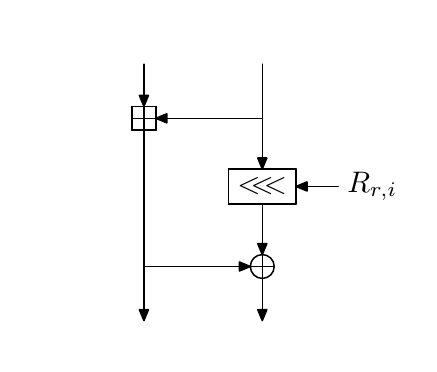
\includegraphics[scale=0.7]{figs/threefish_mix_function.png}
\caption{تابع MIX}
\label{threefish_mix_function}
\end{figure}

\ref{threefish_mix_function}
 نحوهٔ عملکرد 
 \lr{Threefish-512}
 را نشان می‌دهد، هر یک از مراحل هفتاد و دوگانهٔ الگوریتم
 \lr{Skein-512}
 از چهار تابع MIX
 به همراه ضرب در یک کلمه ۶۴ بیتی انجام می‌شوند. ثابت‌های چرخش به شکلی انتخاب می‌شوند تا پخش‌شدگی را در هش به حداکثر خود برسانند. 
 برای به دست آوردن مقدار 
\lr{Threefish-512}
۷۲ بار الگوریتم شکل
\ref{threefish_block_cipher}
تکرار می‌شود.
\footnote{برای مطالعه جزیی‌تر می‌توانید به 
\cite{main_doc}
مراجعه کنید.}

\begin{figure}
\centering
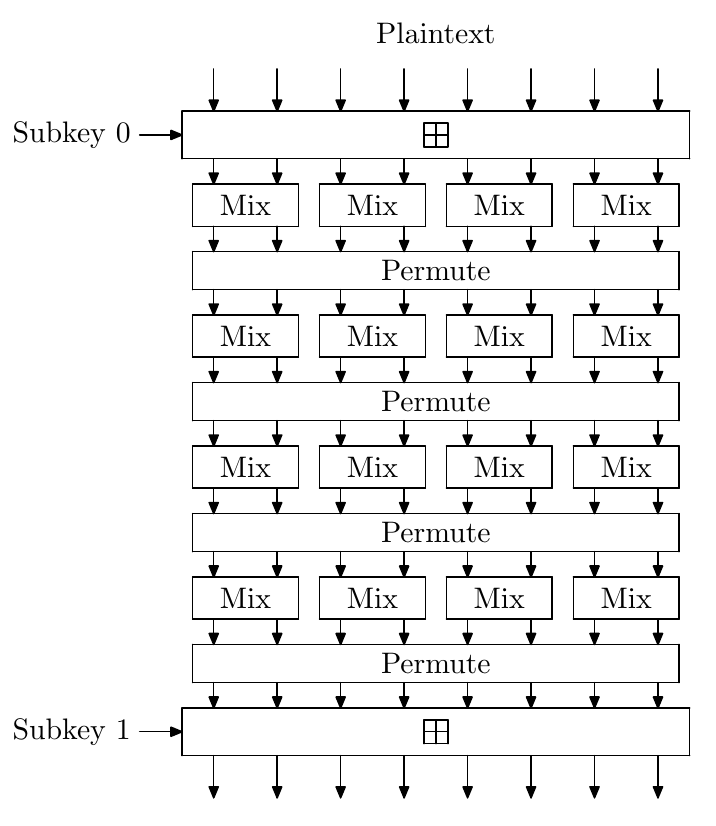
\includegraphics[scale=0.7]{figs/threefish_block_cipher.png}
\caption{چهار مرحله از ۷۲ مرحلهٔ 
\lr{Threefish-512 block cipher}}
\label{threefish_block_cipher}
\end{figure}


\subsection{\lr{Unique Block Iteration}}
\lr{Unique Block Iteration} 
یا به اختصار 
UBI
زنجیره‌ای از ورودی‌ها را با یک رشته با طول دلخواه تلفیق می‌کند تا یک خروجی با اندازهٔ مورد نظر و ثابت به دست آورد، در حقیقت 
UBI
مقدار 
\lr{The Threefish block cipher}
را که مقداری با اندازهٔ نامشخص و تعیین‌نشده‌ست را به خروجی با مقداری با اندازهٔ ثابت تبدیل می‌کند، شکل 
\ref{three_block_message}
نحوهٔ محاسبه 
UBI
برای الگوریتم 
\lr{Skein-512}
را نشان می‌دهد، اندازهٔ ورودی ۱۶۶ بایت است که در سه بلوک ریخته شده است، بلوک‌های 
$M_0$
و 
$M_1$
هر کدام ۶۴ بایت دارند و 
$M_2$ 
که برچسب آخرین بلوک
\footnote{\lr{final block}}
را دارد باقی‌مانده اندازه یعنی ۳۸ بایت دارد. با استفاده از 
tweak
بلوک که قلب اصلی 
UBI
را تشکیل می‌دهد
UBI 
متوجه می‌شود که آیا تمامی بلوک‌ها برای ایجاد خروجی پردازش شده اند یا خیر و این که آیا به بلوک پایانی (پایان زنجیره) رسیده است یا خیر. 
UBI 
یکی از انواع 
\lr{ Matyas-Meyer-Oseas}
ها است.
\cite{matyas}
\begin{figure}
\centering
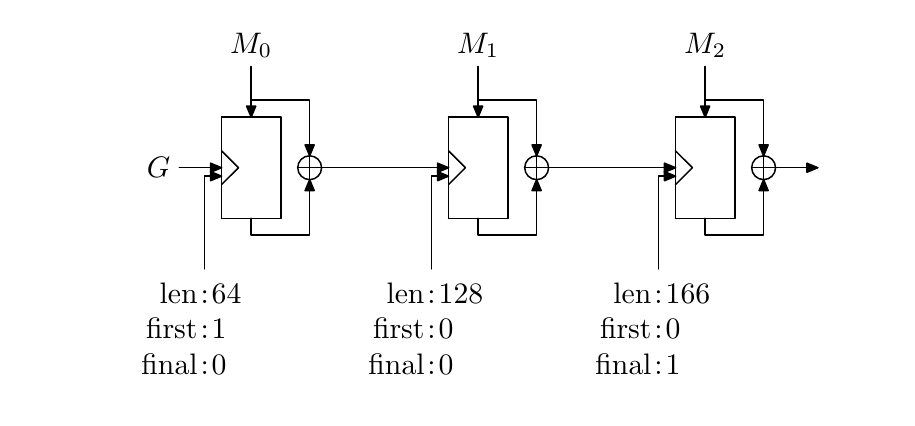
\includegraphics[width=\textwidth]{figs/three_block_message.png}
\caption{درهم‌سازی پیام سه بلوکه  با UBI}
\label{three_block_message}
\end{figure}

\subsection{تابع درهم‌سازی Skein}
تابع اصلی درهم‌سازی در حالت نرمال که مد نظر این نوشتار است برای ایجاد هش از چندین درخواست از 
UBI
و باالتبع از 
\lr{Threefish block cipher}
هش یک داده ورودی را حساب می‌کند، برای محاسبه هش سه بار UBI با ورودی‌های مختلف زیر صدا زده می‌شود، شکل 
\ref{skein_hash}
توضیحات زیر را به صورت شماتیک نشان می‌دهد. 
\begin{itemize}
\item
\textbf{\lr{Config}
}این ورودی مقدار اندازه خروجی و تعدادی از پارامتر‌ها برای 
\lr{Tree-hashing}
را فراهم می‌کند، در صورتی که از حالت استاندارد و نرمال 
Skein 
براش درهم‌سازی استفاده شود این مقدار قابل پیش‌پردازش است.

\item
\textbf{\lr{Message}
}مقدار داده ورودی‌ست.
\textbf{\item{Counter}
}شمارنده‌ای برای نشان دادن تعداد بار تکرار الگوریتم ایجاد خروجی برای رسیدن به خروجی با اندازه مورد نظر است، در صورتی که خروجی بیش از اندازه‌ای مورد انتظار باشد، دوباره تابع ایجاد خروجی فراخوانی می‌شود. 
\end{itemize}
\begin{figure}[h]
\centering
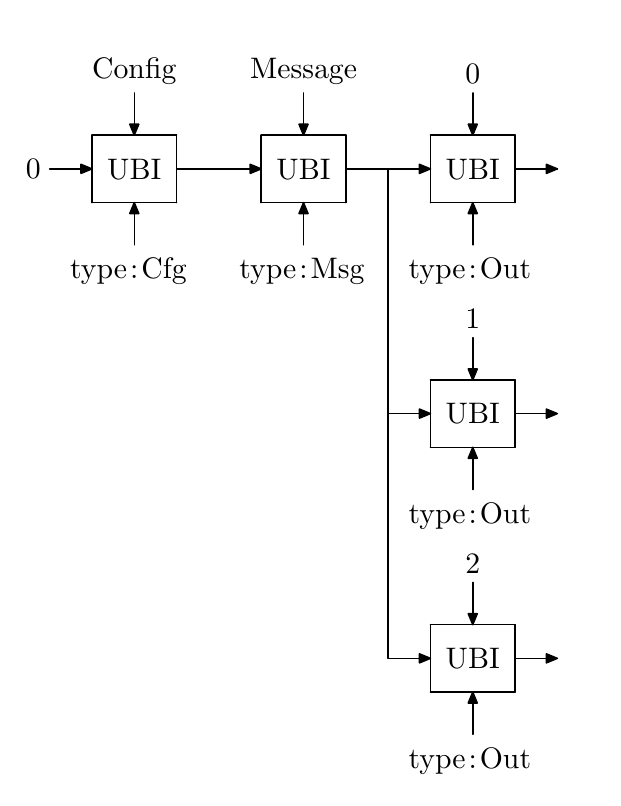
\includegraphics[scale =.5]{figs/skein_hash.png}
\caption{تابع ایجاد هش با خروجی بزرگ‌تر از اندازه مورد انتظار}
\label{skein_hash}
\end{figure}

\subsection{\lr{Optional Arguments}}

در راستای افزایش انعطاف‌پذیری الگوریتم درهم‌سازی skein برای کاربردهای مختلف تعدادی ورودی به صورت اختیاری به الگوریتم افزوده شده اند، در ادامه مختصرا به توضیح ایشان می‌پردازیم. 
\begin{itemize}
\item
\textbf{\lr{Key}}
(اختیاری)
کلیدی برای تبدیل skein
به تابع MAC یا KDF.
\item
\textbf{\lr{Configuration}}
(اجباری)
همان مقدار Config که پیش‌تر توضیح داده شد. 
\item
\textbf{\lr{Personalization}}
(اختیاری)
رشته‌ای که برنامه میتواند با استفاده از آن تابع‌های مختلفی برای کاربردهای مختلفی بسازد. 
\item
\textbf{\lr{Nonce}
}(اختیاری)

مقدار Nonce برای استفاده در حالت 
\lr{stream cipher}
و حالت درهم‌سازی تصادفی.
\item
\textbf{\lr{Message}
}
(اختیاری)

ورودی نرمال تابع درهم‌‌سازی.

\item
\textbf{\lr{Output}
}(اجباری)
مقدار خروجی الگوریتم. 
\end{itemize}

\textit{در محاسبه هش تابع درهم‌سازی 
Skein
به ترتیب ذکر شده در بالا 
UBI
ورودی‌ها محاسبه می‌شود.
}



\section{کاربردهای الگوریتم درهم‌سازی Skein}
\begin{itemize}

\item \textbf{Skein به عنوان تابع درهم‌سازی}
ساده‌ترین راه استفاده از الگوریتم Skein استفاده به عنوان تابعی برای به دست آوردن هش ورودی‌ست، در این حالت Skein مانند تمام الگوریتم‌های دیگر درهم‌سازی عمل می‌کند و رشته‌ای را به عنوان هش با اندازه ازپیش‌تعیین‌شده خروجی می‌دهد.
\item \textbf{Skein به عنوان MAC}
	از تابع درهم‌سازی Skein می‌توان برای تولید MAC
\footnote{\lr{Message authentication code}}
استفاده کرد، از 
MAC 
برای وارسی این که یک پیام از یک فرستنده معتبر بدون تغییر ارسال شده یا که در طی مسیر دست‌کاری شده است استفاده می‌شود. 
\item \lr{\textbf{HMAC}}
\item \textbf{\lr{Randomized Hashing}}
\item \textbf{\lr{Digital Signatures}}
\item \textbf{\lr{Key Derivation Function (KDF)}}
\item \textbf{\lr{Password-Based Key Derivation Function (PBKDF)}}
\item \textbf{\lr{PRNG}}
\item \textbf{\lr{Stream Cipher}}
\end{itemize}
\begin{thebibliography}{1}


\bibitem{skein}{
\lr{
http://www.skein-hash.info/about\\
  }}
  
  \bibitem{main_doc}
  \lr{The Skein Hash Function Family\\
Version 1.3 — 1 Oct 2010\\
http://www.skein-hash.info/sites/default/files/skein1.3.pdf\\
}

  
  \bibitem{matyas}
  \lr{ S.M. Matyas, C.H. Meyer, and J. Oseas, “Generating strong one-way functions with crypto-
graphic algorithms\\” IBM Technical Disclosure Bulletin, Vol. 27, No. 10A, 1985, pp. 5658–5659.\\
}


\end{thebibliography}
